
\documentclass[10pt,conference]{IEEEtran}
\usepackage[utf8]{inputenc}
\usepackage[T1]{fontenc}
\usepackage{amsmath,amssymb}
\usepackage{graphicx}
\usepackage{booktabs}
\usepackage{multirow}
\usepackage{array}
\usepackage{url}
\usepackage[hidelinks]{hyperref}
\setlength{\textfloatsep}{4pt plus 1pt minus 1pt}
\setlength{\floatsep}{4pt plus 1pt minus 1pt}
\setlength{\intextsep}{5pt plus 1pt minus 1pt}
\setlength{\abovecaptionskip}{3pt}
\setlength{\belowcaptionskip}{0pt}
\renewcommand{\arraystretch}{0.94}
\setlength{\parskip}{0pt}
\hyphenpenalty=1000
\sloppy
\begin{document}
\title{\vspace{-1.2em}\normalsize THE UNIVERSITY OF LAHORE $\bullet$ DEPARTMENT OF INTELLIGENT SYSTEMS $\bullet$ AI-101\\[2pt]
\Large Task B1: Detecting Fraudulent Job Postings}
\author{\normalsize Rizwan Ali \quad|\quad Roll No.\ 70177926 \quad|\quad Section A\\
\normalsize\url{https://github.com/RaeesRizwan09/AI101-ML-Assignment-70177926} \quad|\quad Instructor: Dr.\ Muhammad Awais, AI Architect}
\maketitle
\vspace{-1.4em}
\begin{center}\small\itshape A linear SVM over TF-IDF plus structured fields reaches F1 0.868 and PR-AUC 0.945 on the fraud class, while an always-``real'' model is 0.952 accurate and finds nothing.\end{center}
\vspace{-0.6em}

\section{Introduction}
Job boards are a soft target: a fake posting costs nothing to publish, harvests CVs and
identity documents, and is often deleted before anyone investigates. EMSCAD was released so
that the \emph{text} of an advertisement could be used as evidence -- fraudulent postings
tend to have an empty or copied company profile and language aimed at extracting money. Only
4.84\% of postings are fraudulent, so an always-``real'' model is
0.952 accurate and useless; and because the evidence is split between
structured metadata (no company logo, no screening questions) and free text (\emph{wire},
\emph{registration fee}), the useful question is how much each contributes and whether
combining them pays.

\section{Problem Statement}
Each posting is a pair $(x^{\text{str}},x^{\text{txt}})$: binary flags, categorical
fields and five free-text fields. With $y\in\{0,1\}$ marking a fraudulent posting, we learn
$f(x^{\text{str}},x^{\text{txt}})\to[0,1]$ estimating $P(y=1\mid x)$ and predict fraud
iff $f(x)\ge\tau$. This is supervised binary classification with a 1:20 imbalance; success is
precision, recall and F1 on the \emph{fraud} class plus PR-AUC (the honest summary under
imbalance), with ROC-AUC for comparability. The threshold encodes a business cost -- how
many genuine postings may be sent to manual review -- so it is set on validation data.

\section{Dataset Used}
Real or Fake Job Posting Prediction (EMSCAD)~\cite{kaggle}, assembled by the University of
the Aegean~\cite{emscad} and used here from the Hugging Face mirror
\path{victor/real-or-fake-fake-jobposting-prediction} (CC0). It contains 17880
postings, 866 fraudulent (4.84\%), each with five free-text fields,
seven categorical fields, three binary flags and a salary range. I dropped \texttt{job\_id}
(an identifier) and \texttt{salary\_range} (84.0\% missing, and
almost exclusively missing for fraudulent postings -- keeping it would leak the label); no rows
were removed. Missing text becomes the empty string and five missingness indicators are added,
so ``profile absent'' is measurable rather than imputed away.

\section{Dataset Statistics}

\begin{table}[t]
\centering
\caption{Dataset statistics. Text columns are concatenated into one field; missing text becomes the empty string so that absence stays observable.}
\label{tab:stats}
\scriptsize
\begin{tabular}{l@{\hspace{2pt}}l@{\hspace{6pt}}l@{\hspace{2pt}}l}
\toprule
Property & Value & Property & Value \\
\midrule
Samples & 17,880 & Fraud / real & 866 (4.84\%) / 17,014 \\
Features (num/cat/text) & 5/7/5 & Train/val/test & 12,516/2,682/2,682 \\
Missing salary\_range & 84.0\% & Missing department & 64.6\% \\
Median words, real / fraud & 359 / 228 & Vocab (4k sample) & 101177 \\
TF-IDF features & 20\,000 & Majority baseline acc. & 0.9516 \\
\bottomrule
\end{tabular}
\end{table}



\begin{figure}[t]
\centering
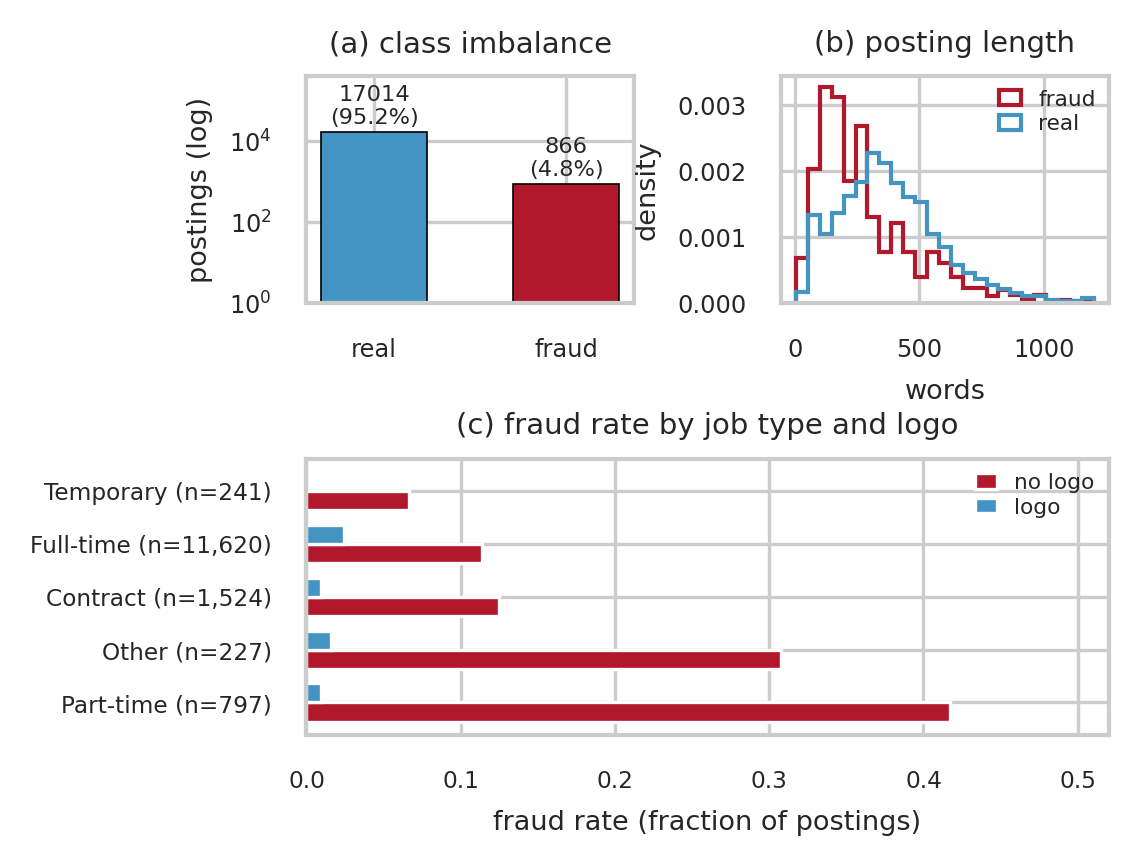
\includegraphics[width=\columnwidth]{figures/B1_fig1_eda.png}
\caption{(a) 1:20 class imbalance; (b) length distribution per class, as a density: fraudulent postings are markedly shorter (median 359 vs 228 words); (c) fraud rate by job type and company-logo presence (bar labels: postings in that job type). A missing logo raises the rate by roughly an order of magnitude in every job type.}
\label{fig:eda}
\end{figure}


\section{Methodology}
\subsection{Learning setting}
Supervised binary classification with severe imbalance. I compared an always-``real''
\emph{Dummy} (a diagnostic: it fixes the accuracy floor), \emph{Logistic Regression}
(linear in a 20k-dimensional TF-IDF space, coefficients readable as evidence),
\emph{Linear SVM} (same space, hinge loss, usually sharper on sparse text) and a
\emph{Random Forest} (non-linear, can exploit interactions between flags and text
frequencies). All three modalities enter one \texttt{ColumnTransformer}:
\texttt{SimpleImputer}+\texttt{StandardScaler} on numeric columns, a
\texttt{OneHotEncoder} (unseen categories ignored) on categorical columns, and
\texttt{TfidfVectorizer} on the concatenated text.

\subsection{Data-split approach}
Stratified 70/15/15 train/validation/test (\texttt{random\_state=42}) gives
12,516/2,682/2,682 postings. Hyperparameters are chosen by 3-fold
\texttt{StratifiedKFold} on the training split, selecting on PR-AUC, which does not reward
the majority class. The threshold is chosen on \emph{validation} to maximise F1 and the test
split is scored once. Imbalance is handled by \texttt{class\_weight='balanced'} inside the
estimator, not by resampling, so no synthetic rows enter the pipeline. Every vectoriser and
encoder is fitted inside the pipeline, hence on training folds only; fitting TF-IDF on the
full corpus would leak test vocabulary.

\subsection{Parameter settings}

\begin{table}[t]
\centering
\caption{Hyperparameters; selection metric is CV PR-AUC on the training split. Shared: word 1--2-gram TF-IDF (min\_df 3, max\_df 0.7, 20k features, sublinear TF) and 266 structured features after one-hot encoding.}
\label{tab:hp}
\scriptsize
\begin{tabular}{>{\raggedright\arraybackslash}p{1.45cm}>{\raggedright\arraybackslash}p{3.35cm}>{\raggedright\arraybackslash}p{1.5cm}}
\toprule
Model & Search space (3-fold CV) & Selected \\
\midrule
Logistic Reg. & $C\in\{0.3,1,3,10\}$, L2, balanced & $C=10$ \\
Linear SVM & $C\in\{0.1,0.5,1,3\}$, balanced & $C=3$ \\
Random Forest & 300 trees, depth $\in\{$-$,30\}$ & no depth limit \\
\bottomrule
\end{tabular}
\end{table}


\section{Results and Analysis}
\subsection{Results}

\begin{table}[t]
\centering
\caption{Test-set results (n=2{,}682, 130 fraud), one evaluation. $\tau$ chosen on validation to maximise F1; fraud is the positive class; best per column in bold.}
\label{tab:res}
\scriptsize
\begin{tabular}{l@{\hspace{3pt}}c@{\hspace{3pt}}c@{\hspace{3pt}}c@{\hspace{3pt}}c@{\hspace{3pt}}c@{\hspace{3pt}}c@{\hspace{3pt}}c}
\toprule
Model & Prec. & Rec. & F1 & PR-AUC & ROC-AUC & Acc. & $\tau$ \\
\midrule
Dummy (always real) & 0.000 & 0.000 & 0.000 & 0.048 & 0.500 & 0.952 & -- \\
RandomForest & 0.765 & 0.800 & 0.782 & 0.879 & 0.988 & 0.978 & 0.34 \\
LogisticRegression & 0.929 & \textbf{0.808} & 0.864 & 0.941 & 0.989 & 0.988 & 0.72 \\
LinearSVM & \textbf{0.938} & \textbf{0.808} & \textbf{0.868} & \textbf{0.945} & 0.988 & 0.988 & 0.13 \\
\bottomrule
\end{tabular}
\end{table}



\begin{figure}[t]
\centering
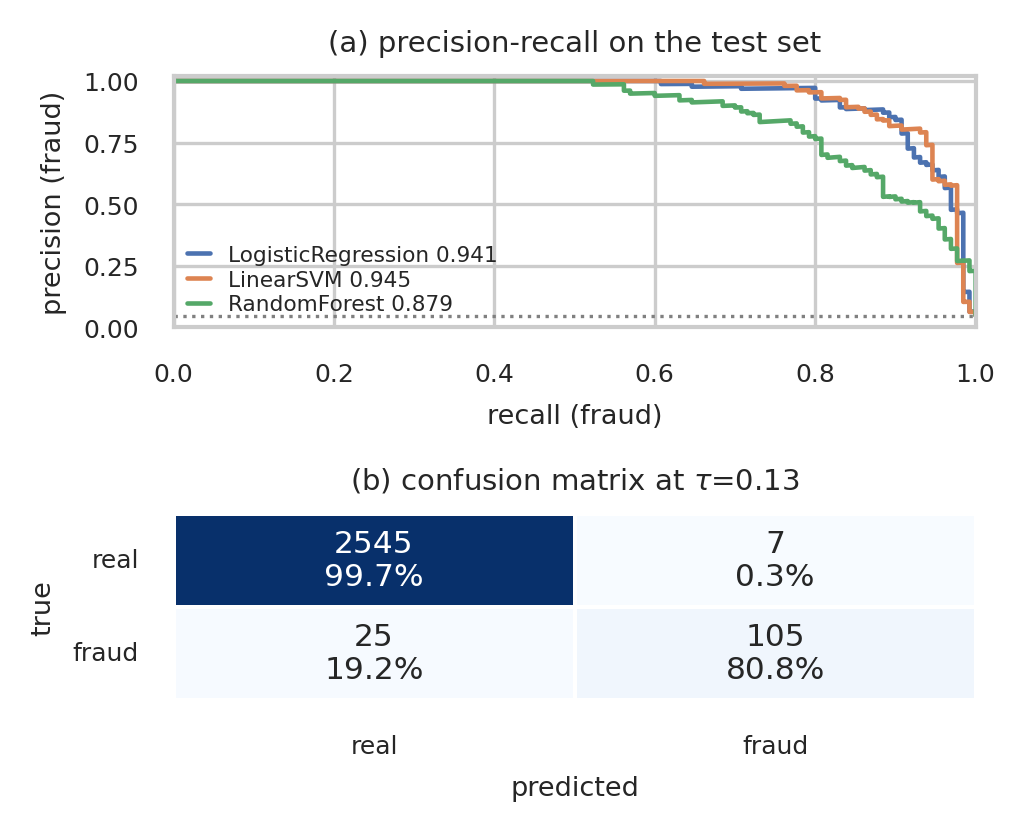
\includegraphics[width=\columnwidth]{figures/B1_fig2_pr_cm.png}
\caption{(a) precision--recall on the test set (legend: average precision); (b) confusion matrix of the best model at its validation-chosen threshold. The dotted line in (a) is the 4.85\% base rate.}
\label{fig:pr}
\end{figure}


\subsection{Analysis}
\textbf{Why accuracy is a poor metric.} The Dummy row settles it: 0.952
accuracy, zero fraud recall, PR-AUC 0.048 -- exactly
the base rate. Accuracy is dominated by the 17014 genuine postings, so a model can look
excellent while never finding a fraud; PR-AUC is the fair summary because its baseline is the
base rate. The best model reaches 0.945, about
19.5$\times$ the base rate.

\textbf{Does combining help?} An ablation answers this. Structured metadata alone
is weak (PR-AUC 0.458,
F1 0.495): a missing logo or profile raises the odds, but most
postings without a logo are genuine small employers. Text alone is nearly as good as the
combined model (PR-AUC 0.928, F1 0.861), and
combining adds +0.017 PR-AUC and
+0.007 F1 over text alone. The gain is small but
consistent and appears mainly in \emph{precision at high recall} -- the region a review queue
operates in.

\textbf{Which words and fields indicate fraud?} The strongest positive TF-IDF weights are
\texttt{link}, \texttt{accion}, \texttt{money}, \texttt{timejob}, \texttt{tester}, \texttt{sales executive}, \texttt{high school}, \texttt{aptitude staffing}; the strongest negative (genuine) weights are \texttt{client}, \texttt{english}, \texttt{exceptional}, \texttt{50}, \texttt{function\_Writing/Editing}, \texttt{prepare} -- exactly the lexicon
a human moderator would use. On the structured side the top weights are \texttt{department\_Product Development}; \texttt{location\_US, CA, }; \texttt{location\_PL, MZ, Warsaw}; \texttt{industry\_Broadcast Media}; these
are one-hot categories with few positives, so some are small-sample artefacts and I would not
report them as findings without confidence intervals. The honest reading is that structured
metadata contributes a prior and the text decides.

\textbf{Error analysis.} At the chosen threshold the model makes 7 false positives
and 25 false negatives out of 130 frauds. Hand-reading the false positives
(``RN Clinical Informatics (near Casper, '' (117 words); ``Finance Assistant'' (169 words); ``Accounting Clerk \$15/hr'' (279 words)) shows the shared failure mode: a genuine posting from a small or new employer
with no logo, a thin company profile and recruiter boilerplate (``apply now'', ``immediate
start'') -- fraudulent on every available signal, but not fraudulent. The false negatives are
postings whose text is lifted almost verbatim from a real advertisement, so the lexical evidence
is absent. That is a label-noise ceiling as much as a modelling one.

\textbf{Limitations.} EMSCAD was annotated around 2014 and fraud language drifts, so absolute
PR-AUC will not transfer to today's boards; the data are also not a random sample of a live
board. Both argue for monitoring precision after deployment.

\section{Conclusion}
Text carries almost all of the signal here (PR-AUC 0.928 alone
versus 0.458 for structured fields), and combining the two
gives the best result at F1 0.868 and PR-AUC 0.945. What did not
work as hoped was the non-linear forest, which trails the linear models on this
high-dimensional sparse space. Next I would test temporal generalisation and calibrate the
score so that "flag for review" maps to a stable expected precision.

\newpage
\section*{AI Use Disclosure}
I used Claude (Anthropic) as an AI assistant for scaffolding this notebook and drafting
report prose from the numbers it produced. The following parts were generated or
substantially assisted by AI: the notebook's cell structure, the plotting code and the first
draft of Sections I--VII. I verified the content by re-running the notebook end to end,
checking that no transformer is fitted outside a \texttt{Pipeline}, confirming that the
threshold is selected on validation only, and reading the top-weighted n-grams by hand to
make sure they are meaningful English rather than artefacts. All experiments, results and
analysis in this report were produced and checked by me, and I take full responsibility for
this work.

\begin{thebibliography}{9}
\bibitem{kaggle} Real or Fake Job Posting Prediction (EMSCAD), Kaggle.
\url{https://www.kaggle.com/datasets/shivamb/real-or-fake-fake-jobposting-prediction}
\bibitem{emscad} S.~Mahbub, E.~Pardede, and A.~Kayes, ``Detection of fraudulent job
advertisements using machine learning,'' 2020.
\bibitem{sklearn} F.~Pedregosa \emph{et al.}, ``Scikit-learn: Machine learning in
Python,'' \emph{JMLR}, vol.~12, pp.~2825--2830, 2011.
\end{thebibliography}
\end{document}
